\section{Optimierung von Reglern}
\subsection{Reglerstrukturen}
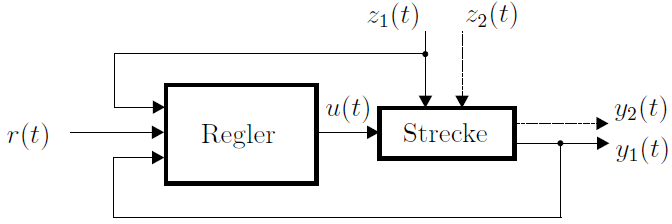
\includegraphics[width=10cm]{./images/Reglerstruktur.png}
\subsubsection{Hierarchische Regelung}
Die verschiedenen Hierarchiestufen unterscheiden sich in einigen Punkten:
\begin{itemize}
	\item Die tiefer liegenden Regler sind ‘klassische’ Regler, die permanent gemäss einer
	Differential- oder Differenzengleichung arbeiten. In höher liegenden Schichten
	werden beispielsweise auch Zustandsautomaten und logische Grössen benutzt.
	\item Soweit man es mit ‘klassischen’ Reglern zu tun hat, arbeiten die tiefer liegenden
	Regler normalerweise mit einer höheren regelungstechnischen Bandbreite $\omega_B$.
	\item Die tiefer liegenden Regler sind meist zeitkritischer. Sie arbeiten mit höherer
	Abtastrate, allenfalls auch analog.
	\item Die oberen Stufen können die unteren Stufen auch steuern und überwachen
	bezüglich Abläufen, Fehlern, Ausfällen, Performance etc.
\end{itemize}

\subsubsection{Kaskadenregelung}
\begin{multicols}{2}
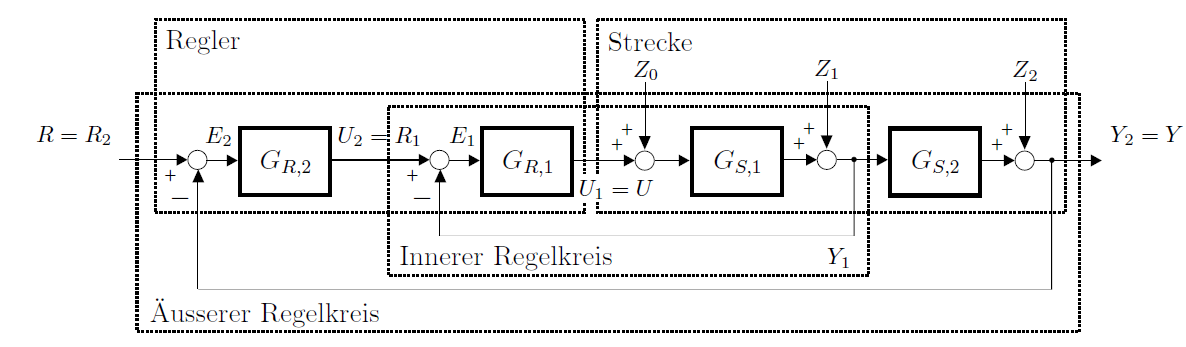
\includegraphics[width=10.5cm]{./images/KaskadenRegelung.png}
Generell gilt bei der Kaskadenregelung folgendes:
\begin{itemize}
\item Beim Reglerentwurf geht man typischerweise von innen nach aussen vor. Zuerst
wird also für die Teilstrecke GS,1 ein Regler GR,1 erstellt. Danach wird für die
fiktive Strecke $G_{S,2} \cdot \frac{G_{S,1}G_{R,1}}{1+G_{S,1}G_{R,1}}$
der Regler GR,2 ausgelegt.
\item Die inneren Regler müssen primär schnell sein; die äusseren Regler dagegen
genau. Mit dem überlagerten Regelkreis kann erzwungen werden, dass der stationäre Fehler verschwindet.
\item Wenn ein innerer Regelkreis gegenüber einem äusseren Kreis schnell ist, dann
erscheint er gegen aussen auch eher als ideales LZI-System. Z.B. kann so das
nichtlineare Verhalten von Leistungshalbleitern gegen aussen versteckt werden.
\item Tendenziell ist die Bandbreite der inneren Regelkreise also grösser zu wählen
als diejenige der äusseren Regelkreise. Dadurch wird eine zeitliche Entkopplung
erreicht; die Regler stören sich gegenseitig weniger.
Normalerweise kann mit der Kaskadenstruktur eine höhere Bandbreite und
auch eine grössere Robustheit erreicht werden gegenüber dem Fall, wenn nur
der äusserste Regelkreis geschlossen wird.
\item Durch die kaskadierte Struktur des Reglers entsteht ein besseres Störverhalten.
Treten in Abb. 103 Störungen bei $z_0$ und $z_1$ auf, reagiert bereits der Regler
$G_{R,1}$ darauf.
\item Entspricht in Abb. 103 der Block GS,2 einem Integrator, dann kann durch die
Messung von $y_1(t) = \dot{y}(t)$ vermieden werden, dass das Signal y(t) im Regler
differenziert werden muss. Dies ist ja gerade bei verrauschten Signalen nicht
zu empfehlen.
\item Natürlich sind die Kosten des zusätzlichen Sensors und seine Integration ins
Regelsystem nachteilig. (Auf Seite der Aktoren ändert sich dagegen nichts.)
\end{itemize}
\end{multicols}

\subsubsection{Störgrössenaufschaltung}


\subsubsection{Vorfilter, Vorsteuerung, 2DOF (Two degrees-of-freedom)}


\subsection{Reglereinstellungen}

\subsubsection{Empirische Einstellregeln nach Ziegler-Nichols}
\begin{tabularx}{0.5\textwidth}{|X||X|X|X|}
\hline
Regler & $K_R$ & $T_N$ & $T_V$ \\ \hline\hline
P-Regler & $\frac{T_g}{K_s\cdot T_u}$ & - & - \\ \hline
PI-Regler & $0.9\cdot\frac{T_g}{K_s\cdot T_u}$ & $3.33\cdot T_u$ & - \\ \hline
PID-Regler & $1.2\cdot\frac{T_g}{K_s\cdot T_u}$ & $2\cdot T_u$ & $0.5\cdot T_u$ \\ \hline
\end{tabularx}

\subsubsection{Optimierung mithilfe eines Gütemasses}

Zur einfacheren Beurteilung der Regelgüte wird die Information der Signale mit einer Zielfunktion auf ein
Gütemass J reduziert.
\begin{eqnarray}
J(k_1,\cdots,k_M)=\int\limits_{0}^{T_{end}}f(e(t,k_1,\cdots,k_M))dt\\
J=\int\limits_{0}^{\infty}e(t)^2dt= \frac{1}{2\pi} \int\limits_{-\infty}^{\infty}|E(j\omega)|^2d\omega= \frac{1}{2\pi} \int\limits_{-\infty}^{\infty}E(j\omega)E^{\ast}(j\omega)d\omega\\
J_1=\frac{b_0^2}{2a_0a_1} \qquad J_2=\frac{b_1^2a_0+b_0^2a_2}{2a_0a_1a_2} \qquad J_3=\frac{b_2^2a_0a_1+(b_1^2-2b_0b_2)a_0a_3+b_0^2a_2a_3}{2a_0a_3(a_1a_2-a_0a_3)} \qquad  \\
Bedingung: Nennerpolynom E(s) muss stabil sein
\end{eqnarray}

\begin{itemize}
\item Die Funktion $f(e)$ wird meist so gewählt, dass $f(\overline{e}) > f(e)$ für $|\overline{e}| > |e|$.
Kandidaten sind z.B. $f(e) = |e| oder f(e) = e^2$ (ISE, integral of squared
error). Grössere Werte von e werden damit ‘bestraft’; je grösser der Wert von
J ist, desto schlechter ist der Regelkreis.
\item Die Dauer $T_{end}$ des ausgewerteten Intervalls muss auf die (zu erwartenden)
Zeitkonstanten des Regelkreises abgestimmt sein. Tend sollte mindestens so
gross sein, dass der Regelkreis bei vernünftiger Reglereinstellung als eingeschwungen
gelten kann.
\end{itemize}

\subsubsection{Vorgabe der Führungsübertragungsfunktion}

Wie kannder Regler bestimmt werden, mit dem das gewünschte $G_f(s)$ resultiert?
Der Regler für eine Strecke $G_S(s) = Z_S(s)/N_S(s)$ und für eine geeignet gewählte
Führungs-UTF $G_f(s) = Z_f(s)/N_f(s)$ kann so berechnet werden:
\begin{equation}
\boxed{G_R(s)=\frac{Z_f(s)}{N_f(s)-Z_f(s)}\cdot\frac{N_S(s)}{Z_S(s)}}
\end{equation}
\begin{itemize}
\item  Die Strecke muss stabil sein. Andernfalls würden in der rechten Halbebene
Pole der Strecke durch Nullstellen im Regler gekürzt, was nicht erlaubt ist.
\item  Wenn die Strecke nicht minimalphasig ist, tritt dasselbe Problem anders herum
auf ausser wenn die nichtminimalphasigen Nullstellen von $G_S$ in $G_f$
übernommen werden, 
\item  Die Strecke darf keine Totzeit haben (Faktor $e^{-sT_t}$ ). Andernfalls müsste im
Regler ein idealer Prädiktor (Faktor $e^{sT_t}$) realisiert werden.
\item  Der relative Grad (d.h. der Polüberschuss) der vorgegebenen UTF $G_f (s)$ muss
mindestens so gross sein wie derjenige der Strecke $G_S(s)$. Andernfalls bekäme
der Regler mehr Nullstellen als Pole, also einen negativen relativen Grad, womit
er nicht realisierbar würde.
\end{itemize}
